\documentclass[a4paper, 11pt]{article}
\usepackage[polish]{babel}
\babelprovide[transforms=oneletter.nobreak]{polish}
\usepackage{titling}
\usepackage{amsmath}
\usepackage[hidelinks]{hyperref}
\usepackage{graphicx}
\usepackage{float}


\title{
   Odczytywanie tablic rejestracyjnych wraz z symulacją płatności za postój na parkingu
}

\date{}


\author{Paweł Strzelczyk}


\begin{document}
\maketitle

\section{Opis projektu}

Celem projektu było stworzenie systemu brzegowego umożliwiającego automatyczne odczytywanie/rozpoznawanie tablic rejestracyjnych (ANPR) samochodu osobowego. Takie rozwiązanie mogłoby być zastosowane na wjeździe/wyjeździe z parkingu płatnego lub o ograniczonym dostępie. 

\section{Architektura}

\subsection{Sprzęt}

W projekcie wykorzystano platformę sprzętową Raspberry Pi 4, kamerę Raspberry Pi Camera HD v3 oraz czujnik tlenku węgla i łatwopalnych gazów MQ-9. 

\subsection{Oprogramowanie}

Aplikacja odpowiadająca na obsługę sprzętu została napisana z wykorzystaniem frameworka Flask w Pythonie. Za jej pośrednictwem udostępniony jest interfejs internetowy wykorzystujący protokół HTTP szyfrowany przy pomocy TLS (HTTPS). Z interfejsu korzysta aplikacja mobilna napisana w frameworku Flutter. Dane przechowywane są w bazie SQL, a do zarządzania nią, wykorzystano system SQLite.

\subsection{Sposób działania}

Wraz z uruchomieniem aplikacji internetowej, uruchamiane są, jako procesy, skrypty odpowiadające za odczyt danych z kamery oraz czujnika. Zależnie od konfiguracji urządzenia, które może służyć jako każdy element parkingu, kamera odpowiada za odczytywanie rejestracji lub skanowanie/detekcję kodu QR celem dokonania płatności. Przyjęto następujące założenia:

\begin{itemize}
\item samochód o danych numerach rejestracyjnych może wielokrotnie korzystać z parkingu,
\item dwa samochody o takich samych numerach rejestracyjnych nie mogą jednocześnie znajdować się na parkingu,
\item postój do 15 minut jest darmowy, dalej każda rozpoczęta godzina płatna,
\item można podjąć próbę wyjazdu bez płacenia (obecnie często występuje płatność ,,na słupku''),
\item numery rejestracyjne są siedmioznakowe.
\end{itemize}

Aplikacja mobilna umożliwia kontrolę stanu parkingu, m.in.:
\begin{itemize}
\item czas ostatniego odczytu przekroczenia poziomu CO lub gazów łatwopalnych,
\item zajętość parkingu,
\item liczbę użytkowników parkingu,
\item sumę opłat za korzystanie, 
\item średnią opłatę za postój,
\item historię postojów,
\item historię odczytów z czujnika.
\end{itemize}


\section{Prezentacja}

\subsection{Link do repozytorium}

\href{https://github.com/pawelstrzelczyk/car-park}{\underline{\LARGE GitHub}}

\subsection{Dokumentacja wizualna}

\begin{figure}[H]
\begin{center}
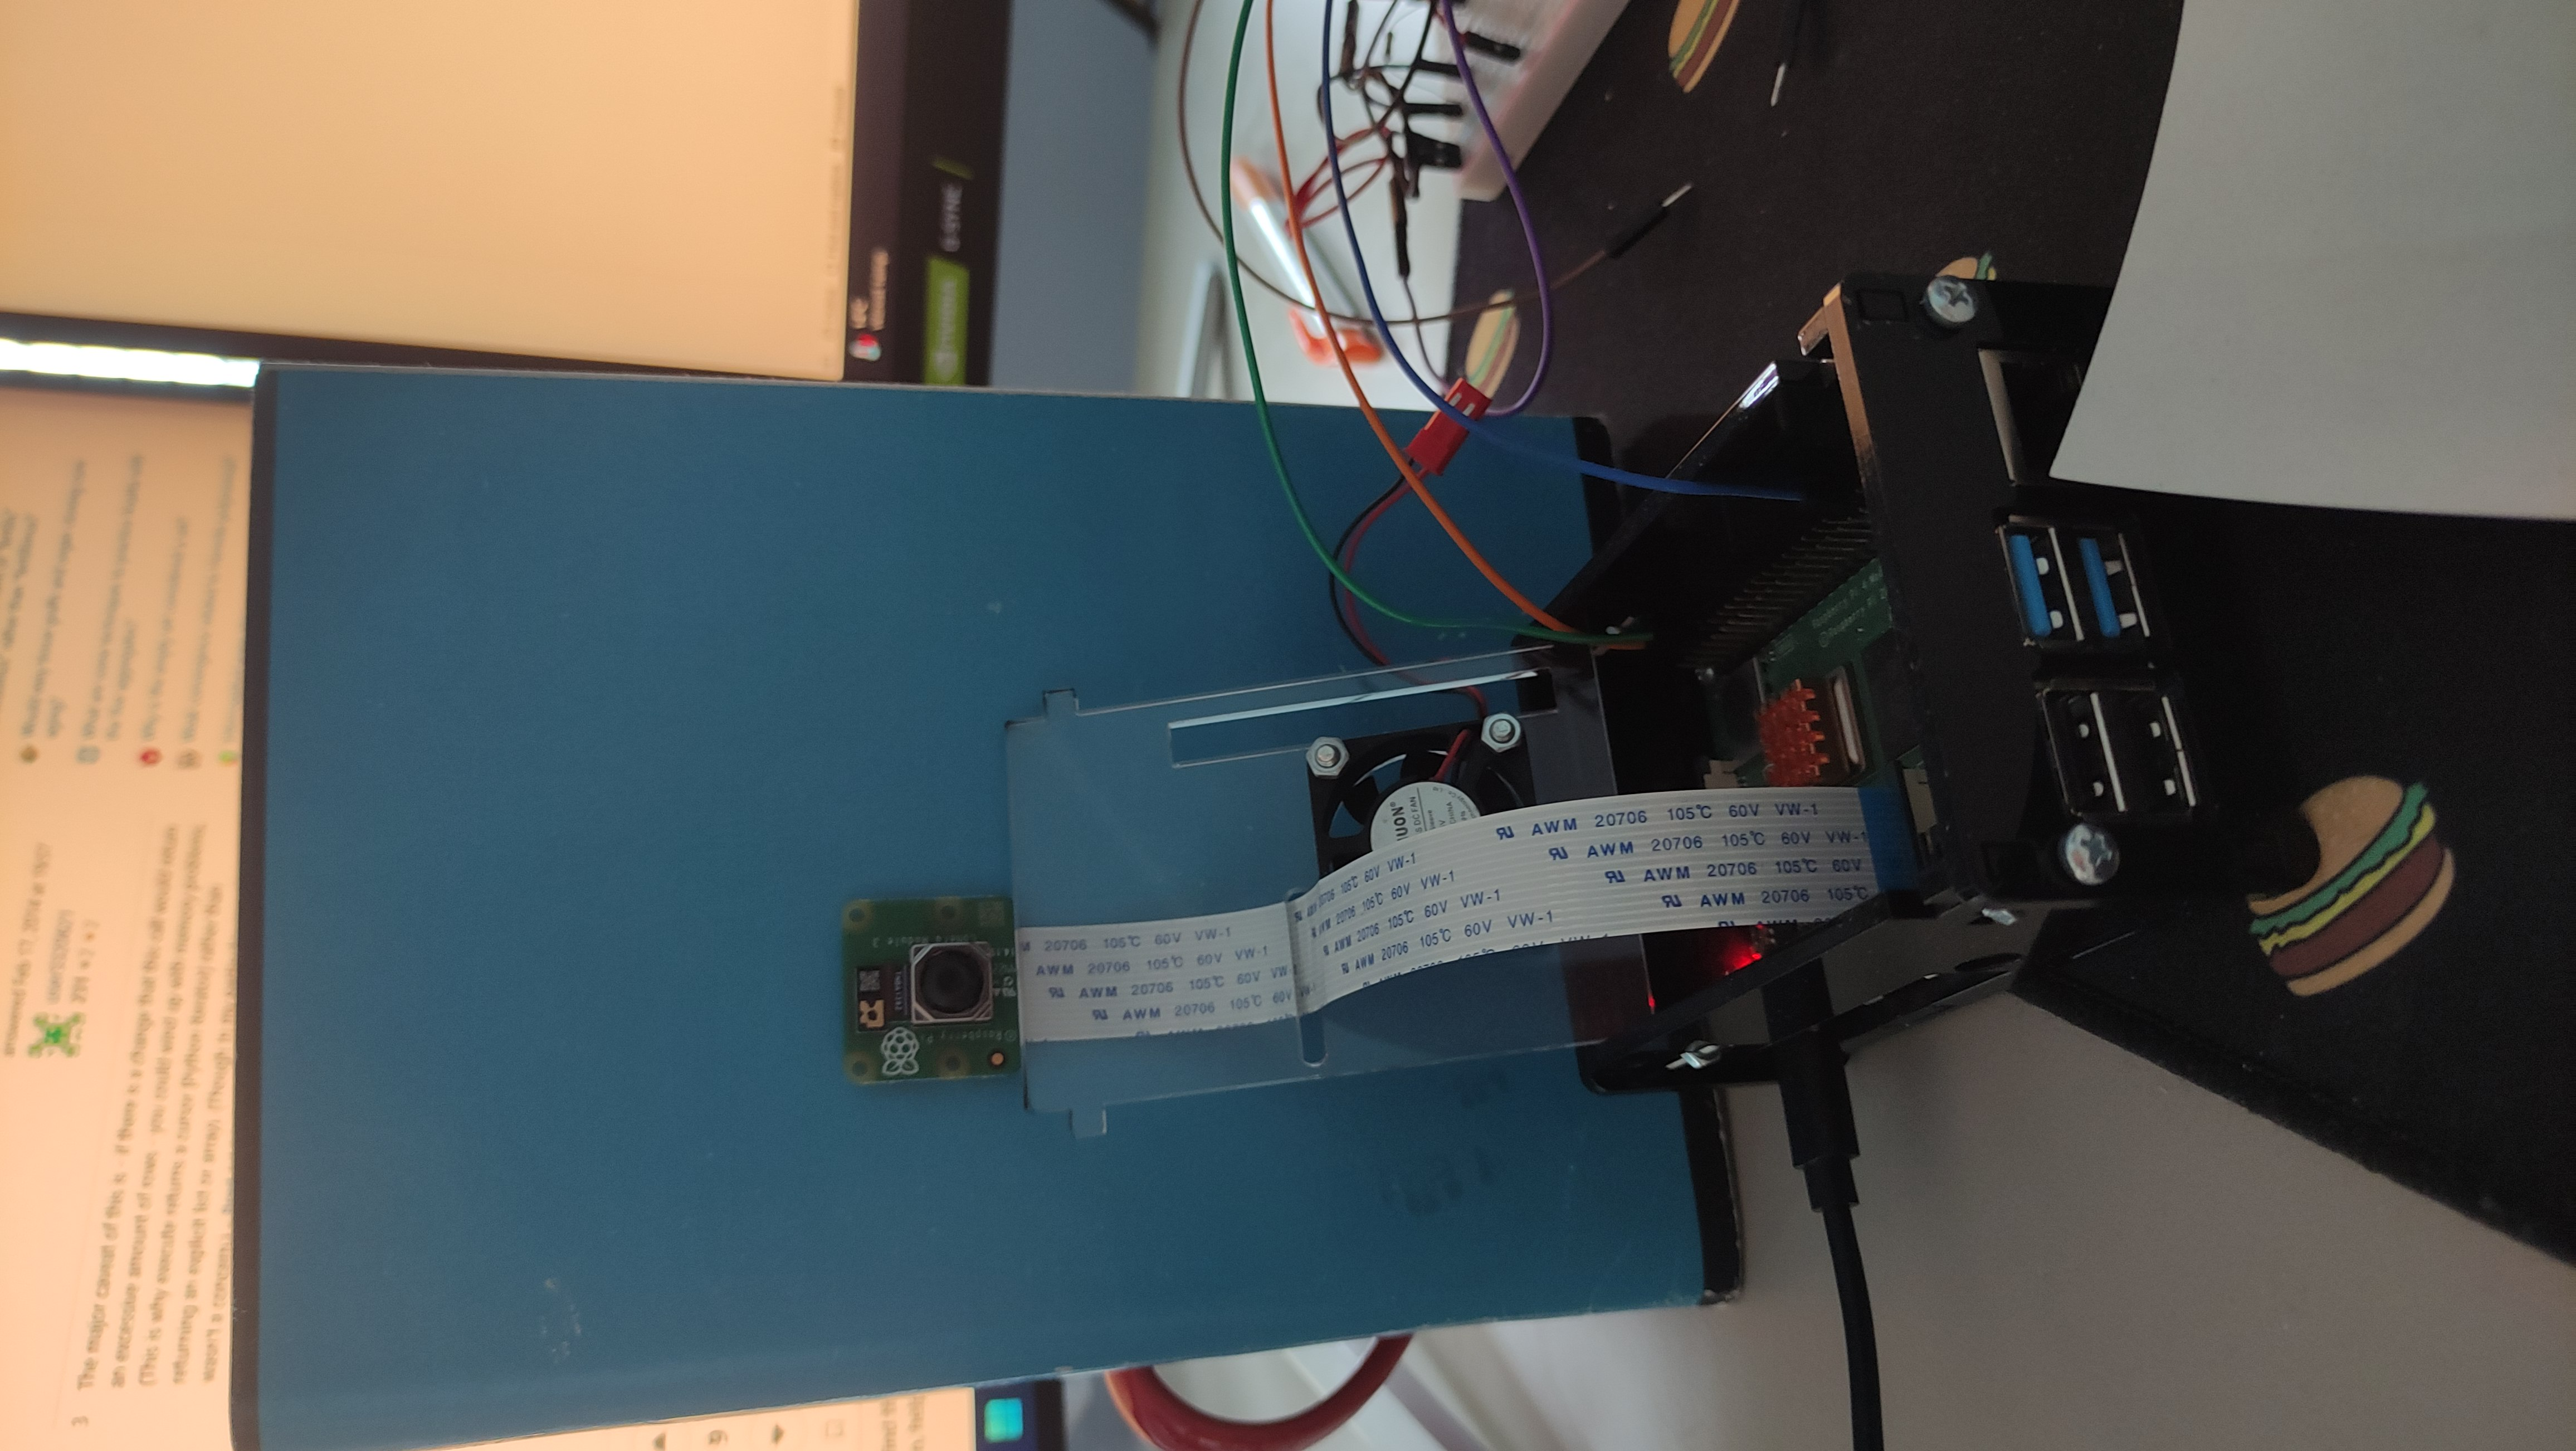
\includegraphics[width=\linewidth]{raspberry.jpg}
\caption{Raspberry Pi 4 z podłączoną kamerą oraz czujnikiem, konstrukcja do demo.}
\end{center}
\end{figure}

\begin{figure}[H]
\begin{center}
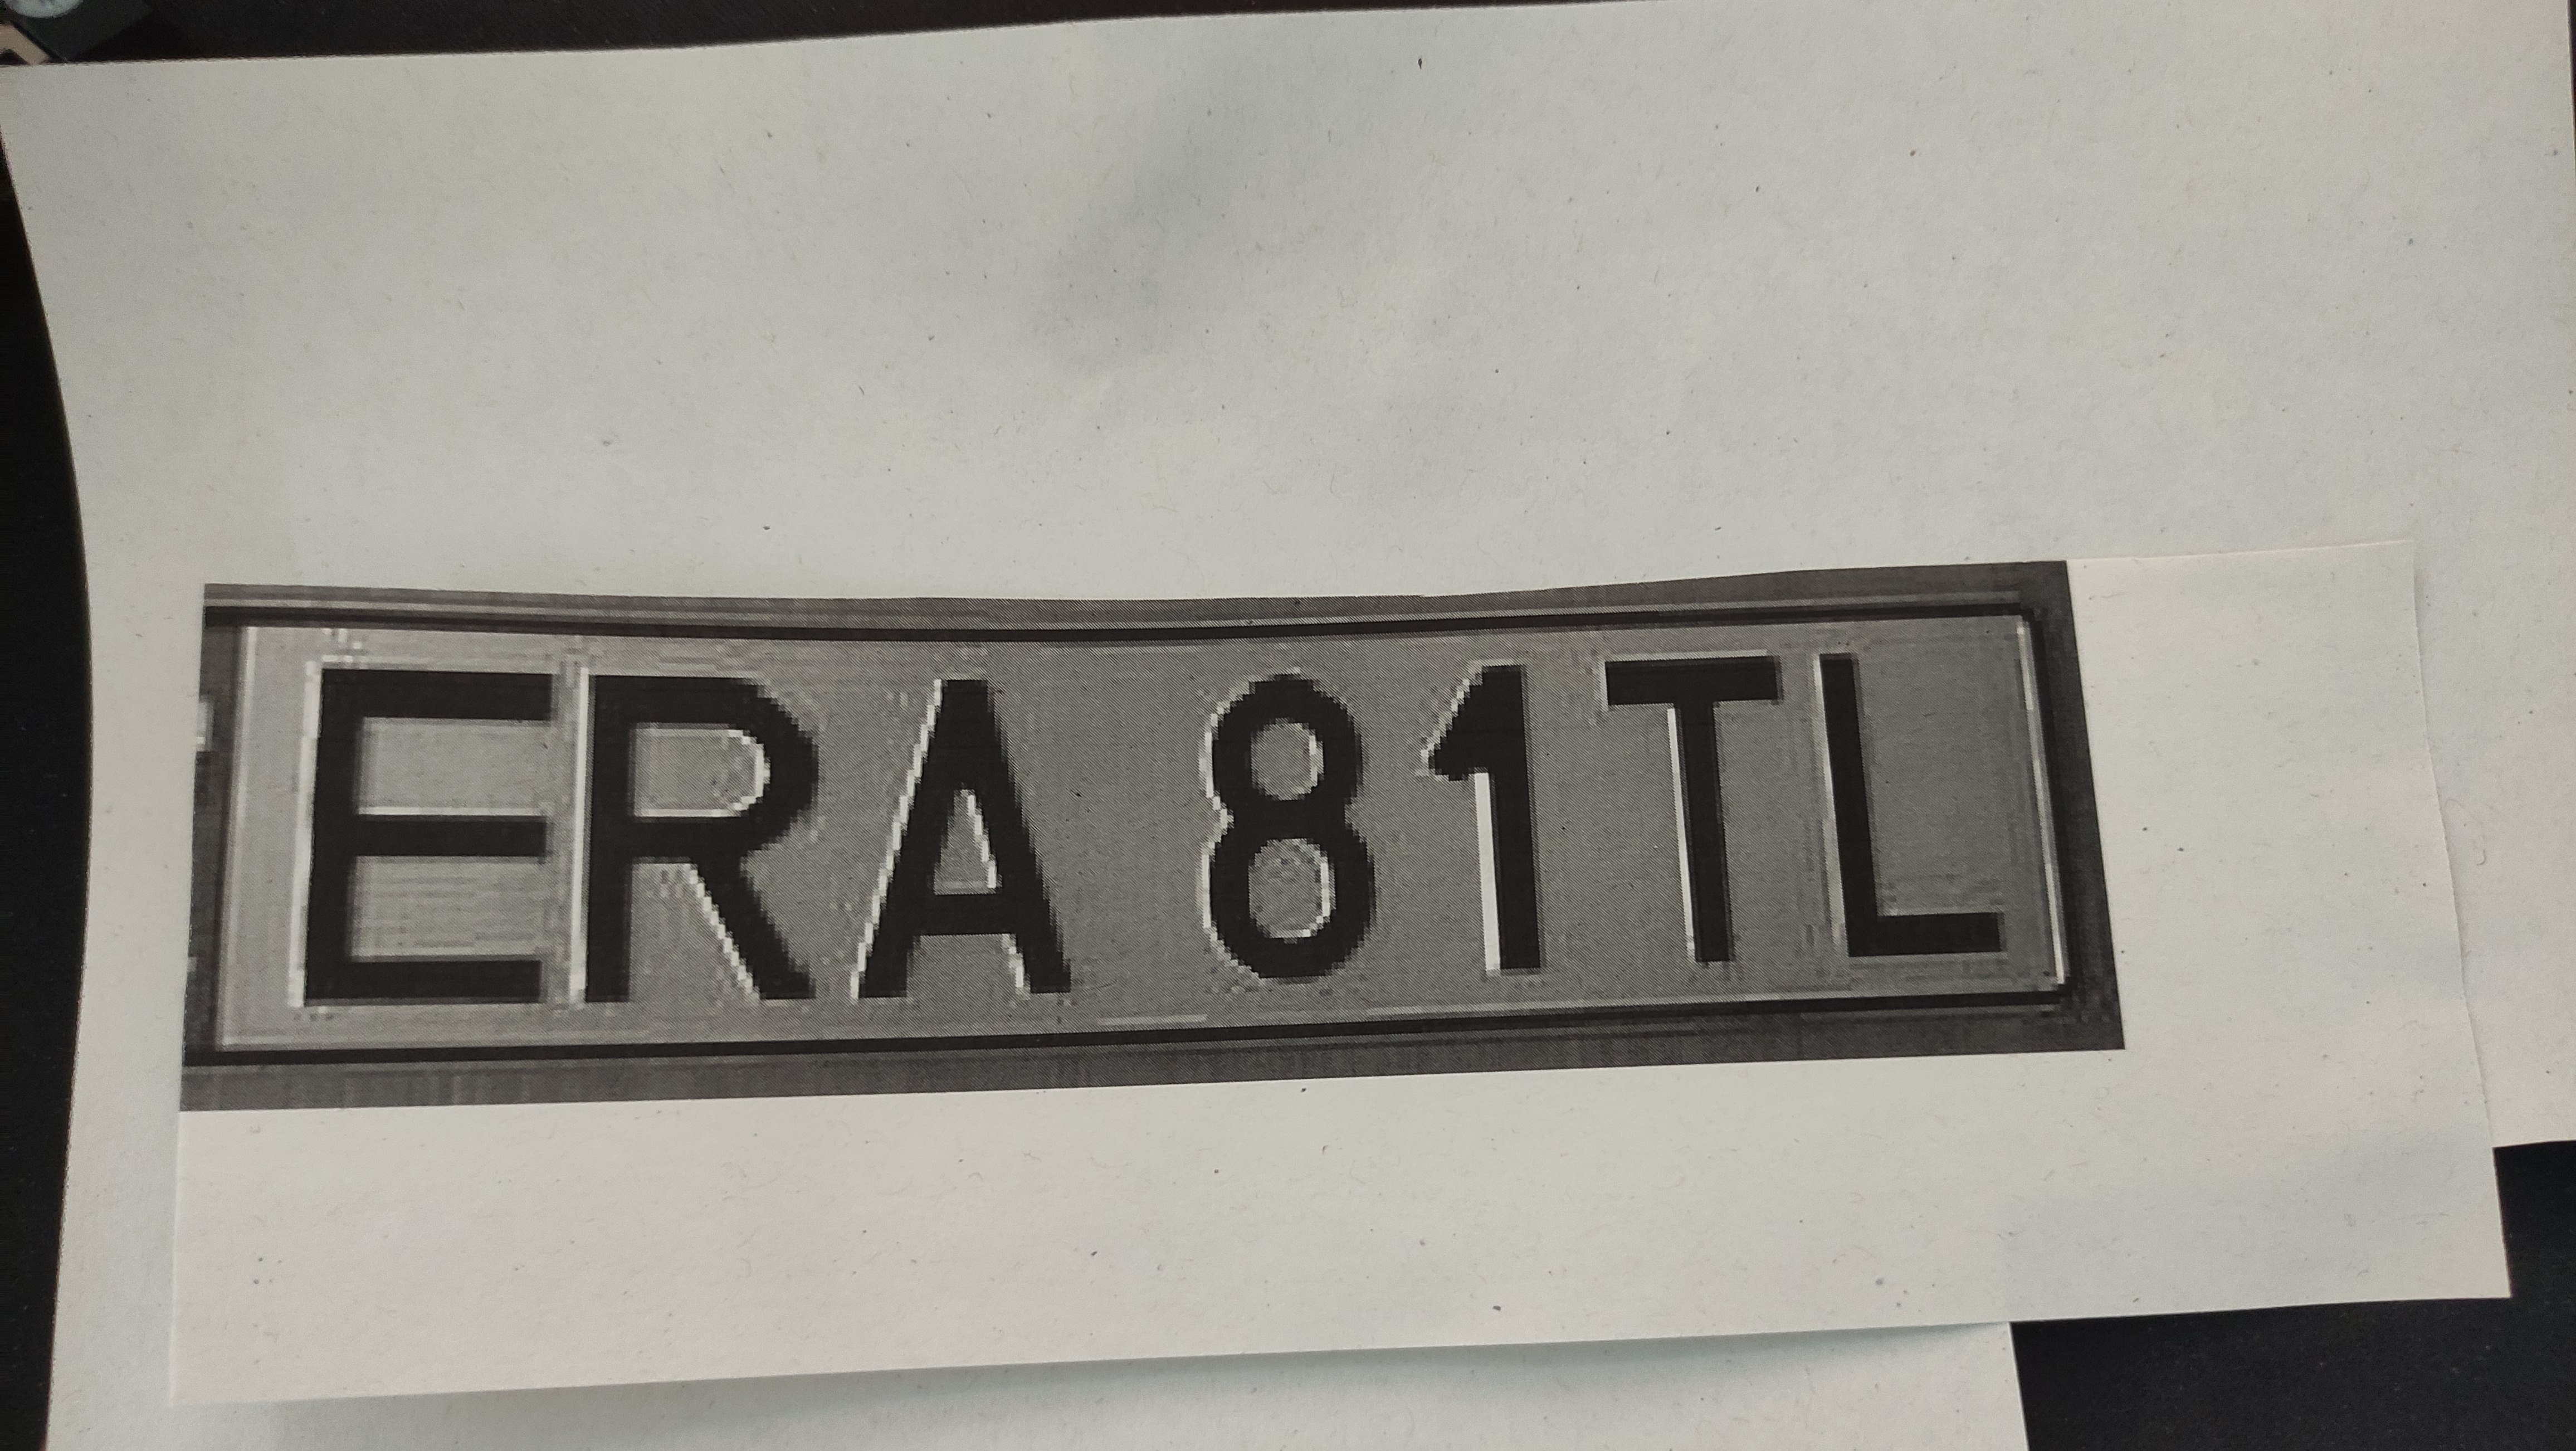
\includegraphics[width=0.6\linewidth]{rejestracja.jpg}
\caption{Wydrukowana rejestracja do demo (film).}
\end{center}
\end{figure}


\begin{figure}[H]
\begin{center}
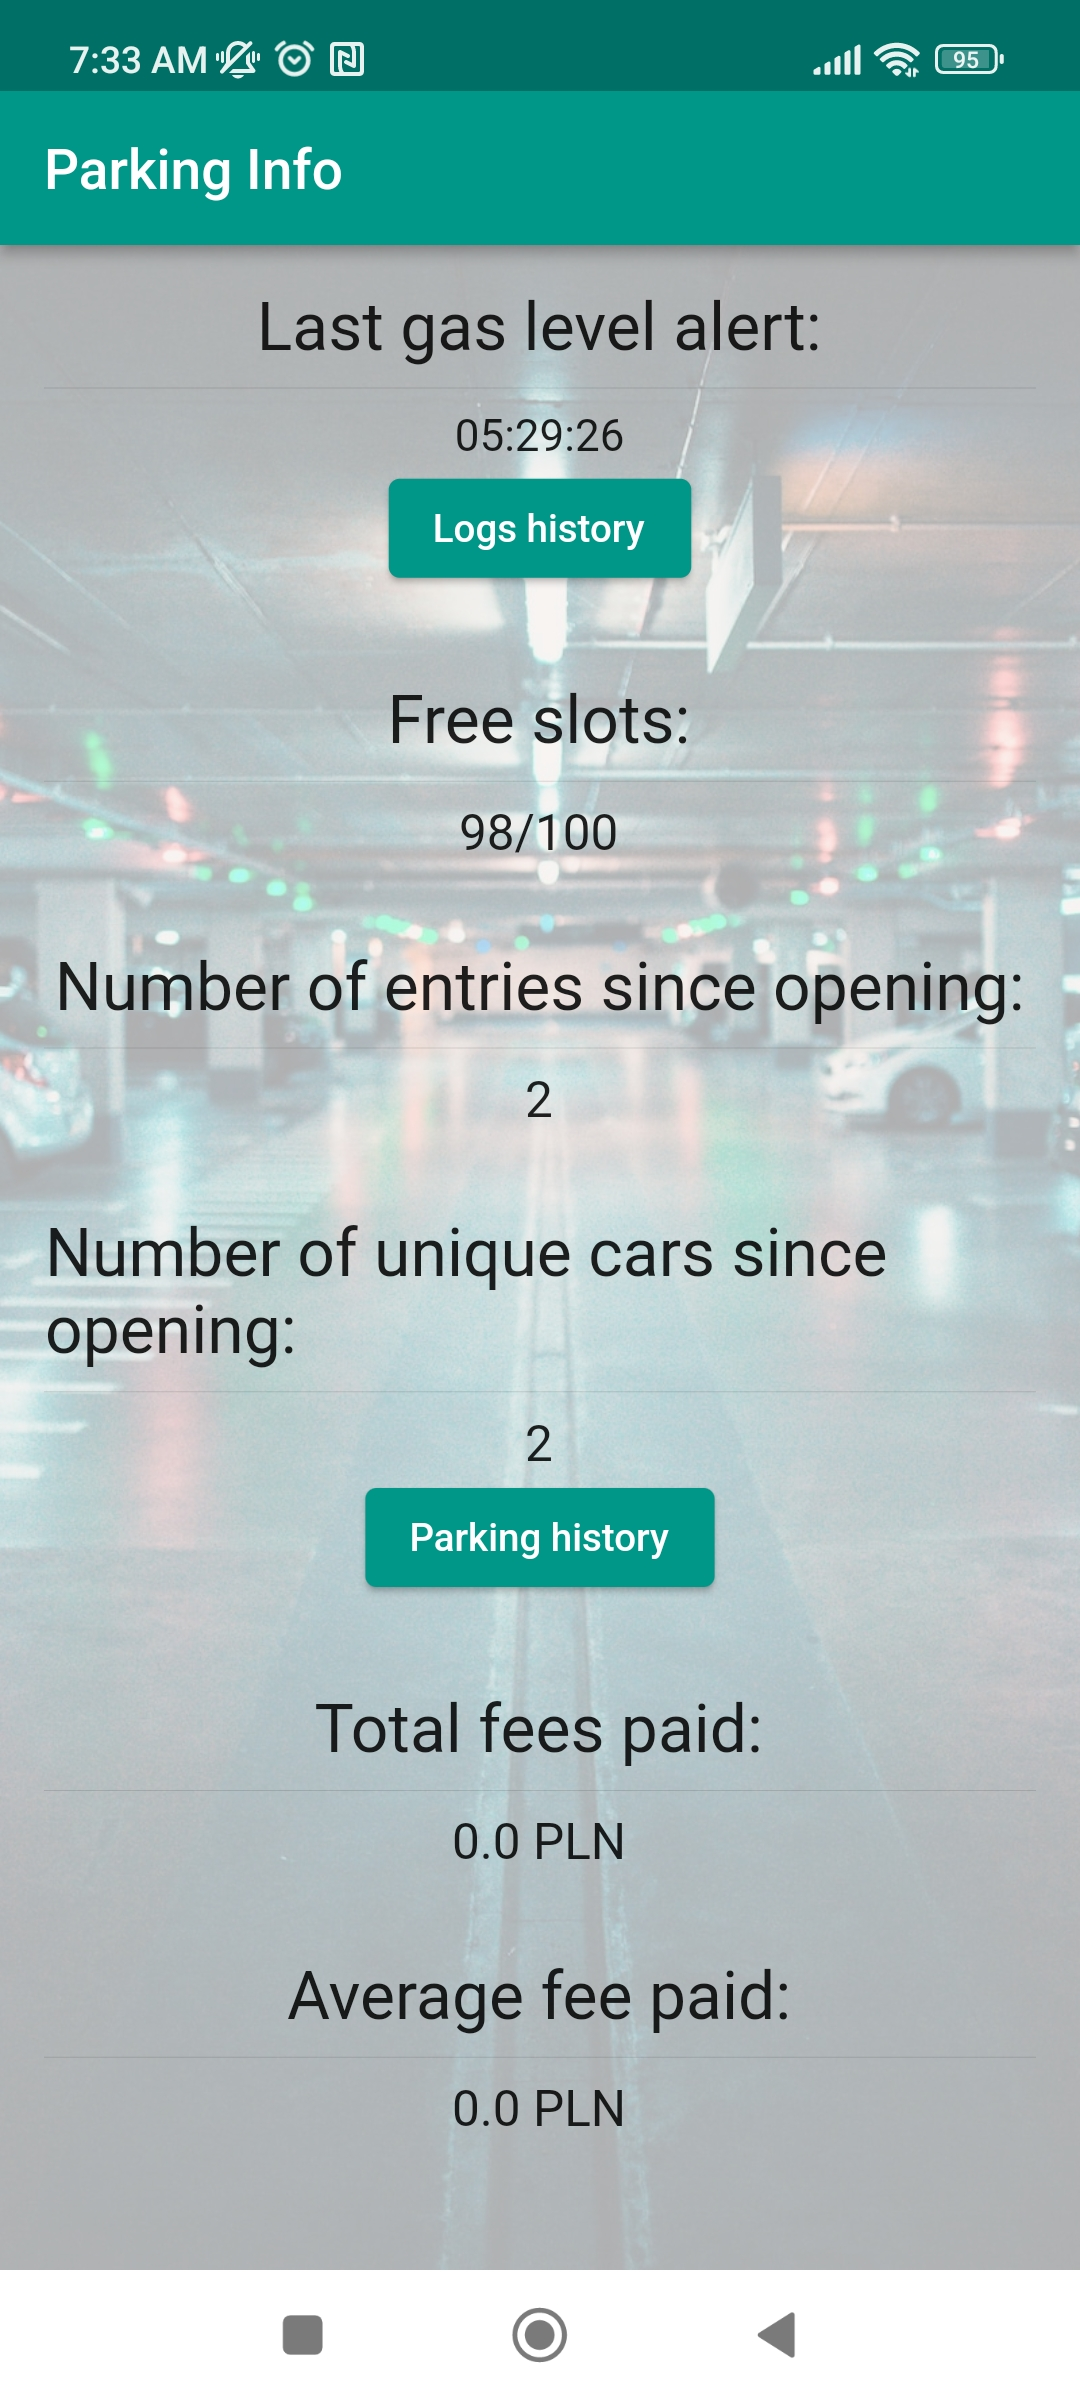
\includegraphics[width=0.6\linewidth]{panel.jpg}
\caption{Główny panel aplikacji.}
\end{center}
\end{figure}


\begin{figure}
\begin{center}
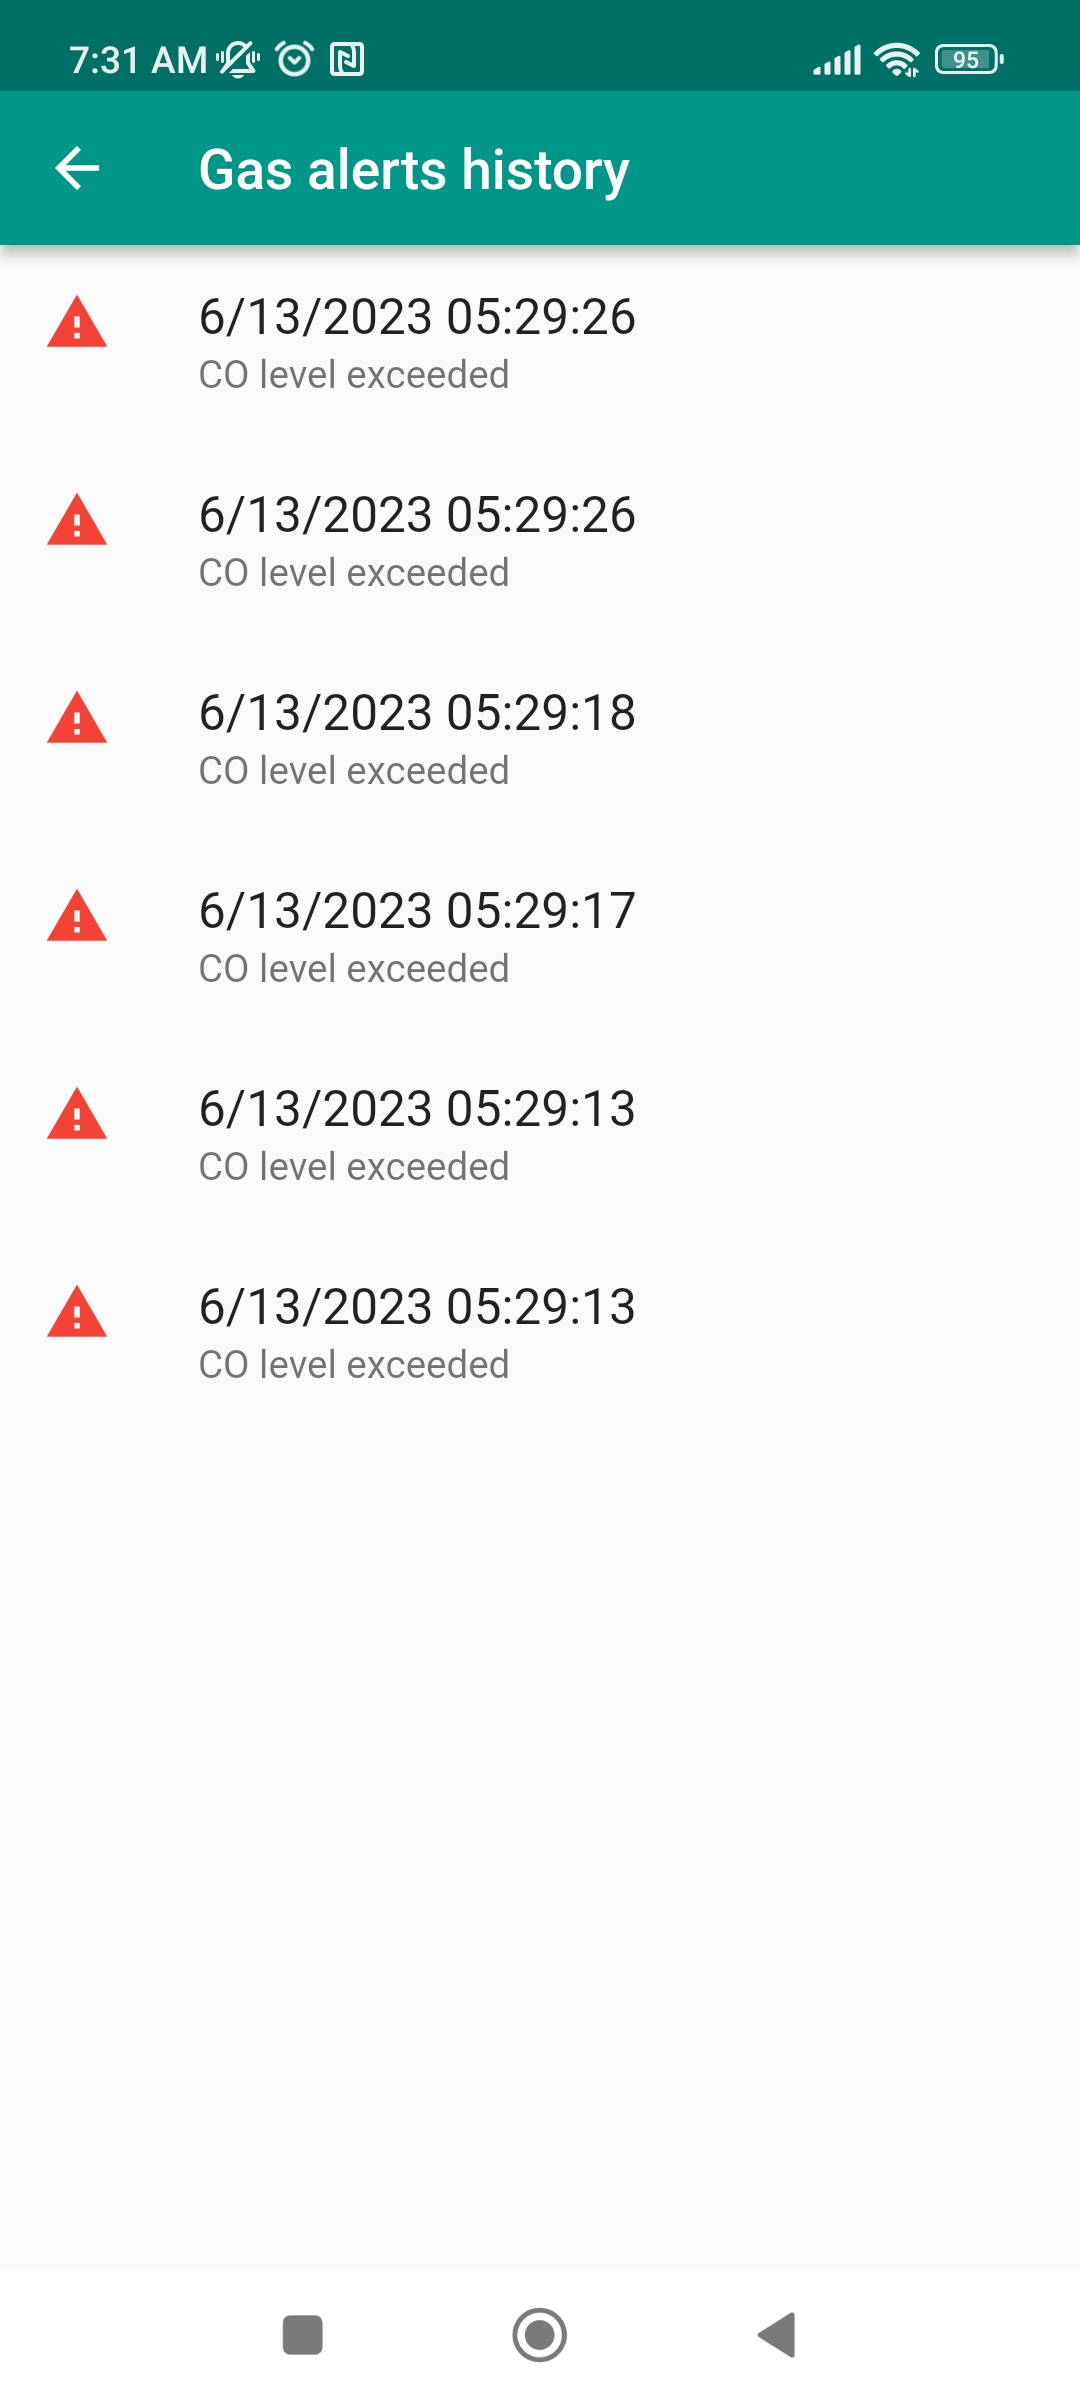
\includegraphics[width=0.6\linewidth]{co.jpg}
\caption{Widok aplikacji z listą odczytów przekroczenia poziomu gazów.}
\end{center}
\end{figure}

\begin{figure}
\begin{center}
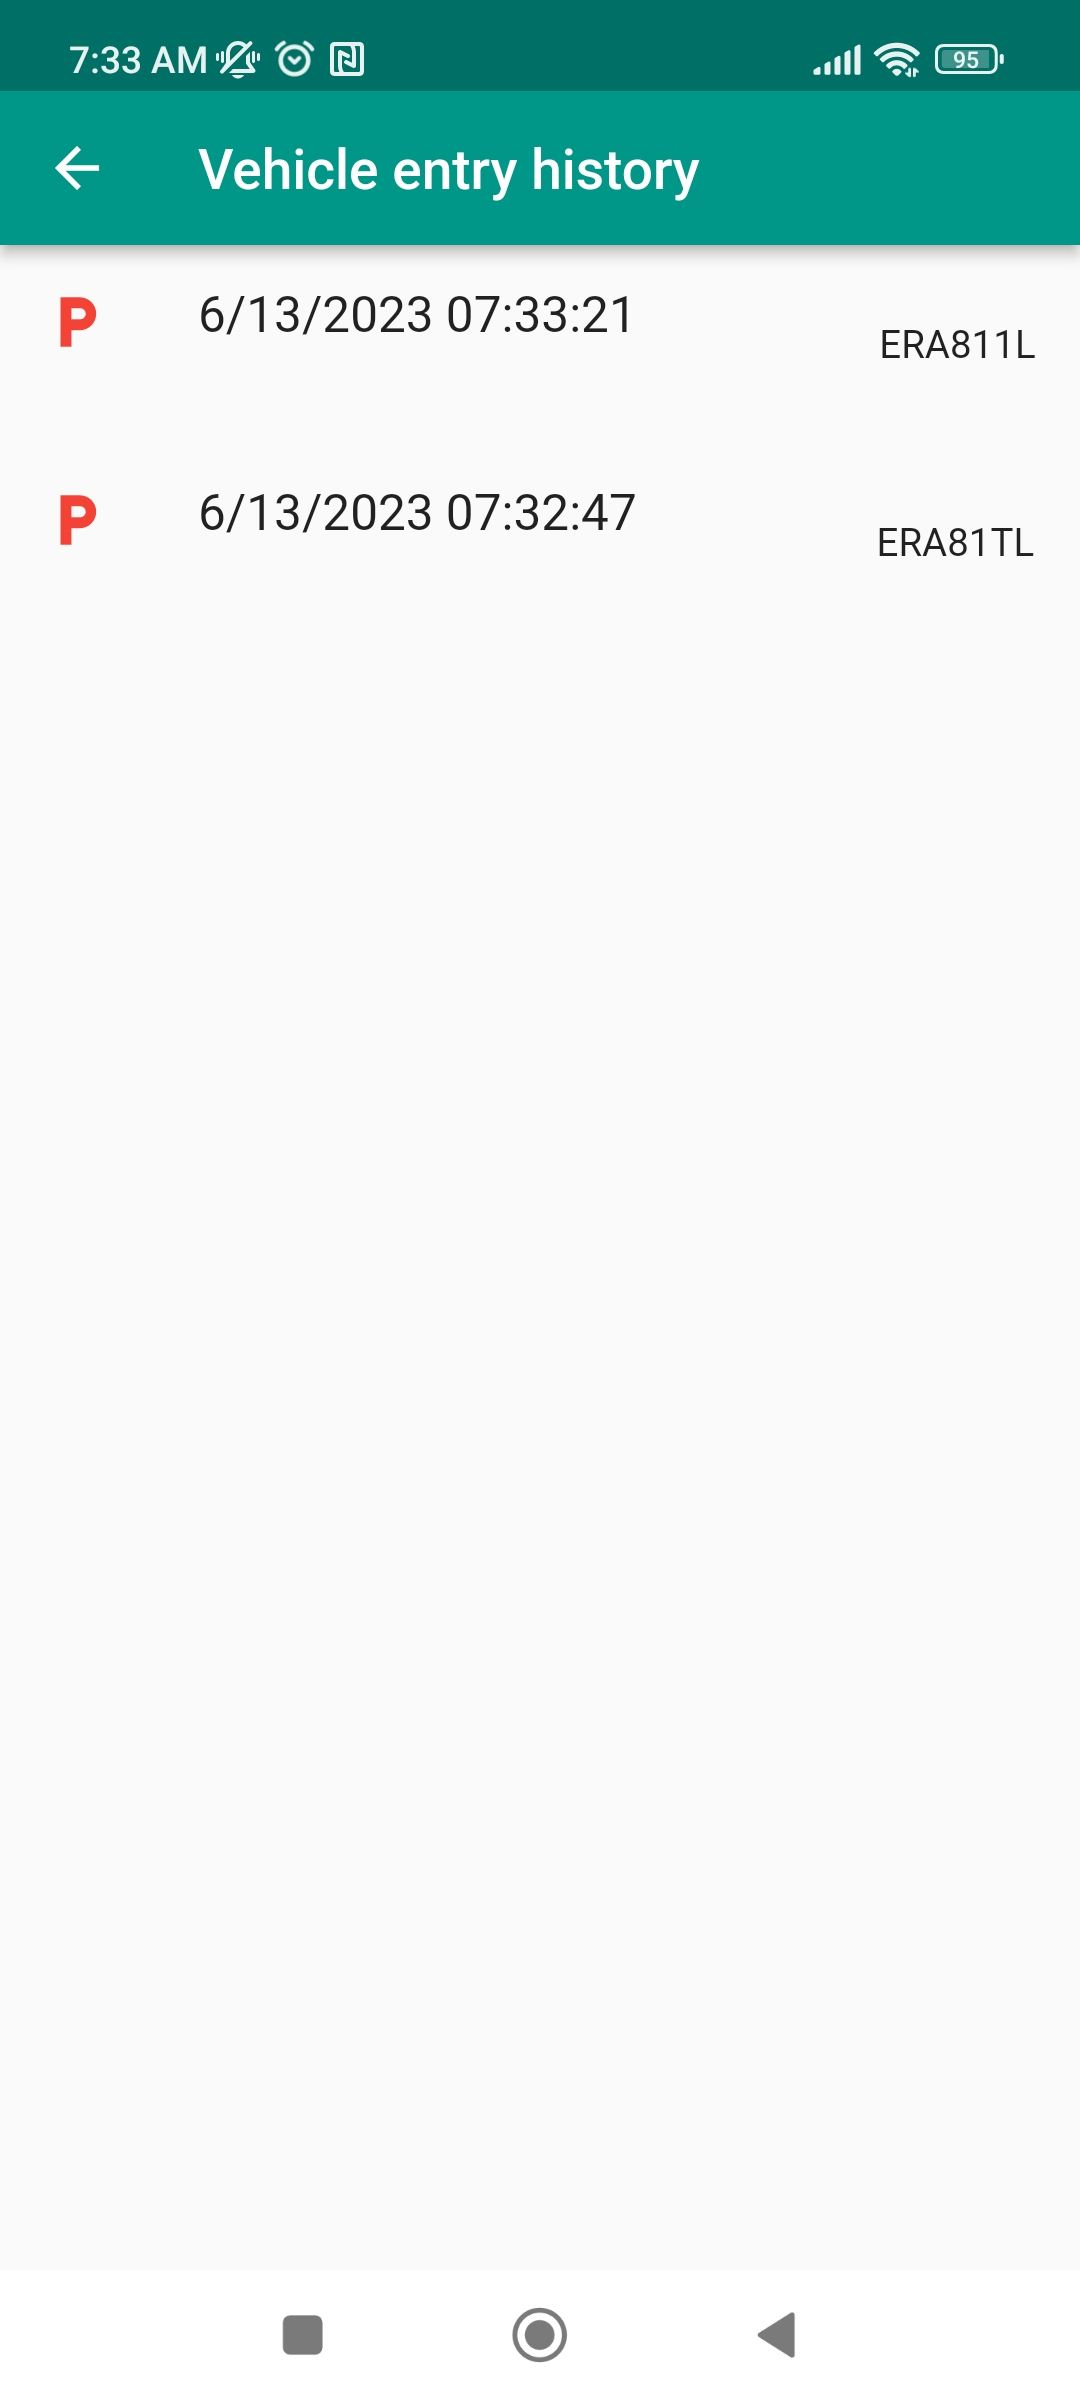
\includegraphics[width=0.6\linewidth]{postoj.jpg}
\caption{Lista pojazdów znajdujących się na parkingu.}
\end{center}
\end{figure}

\begin{figure}
\begin{center}
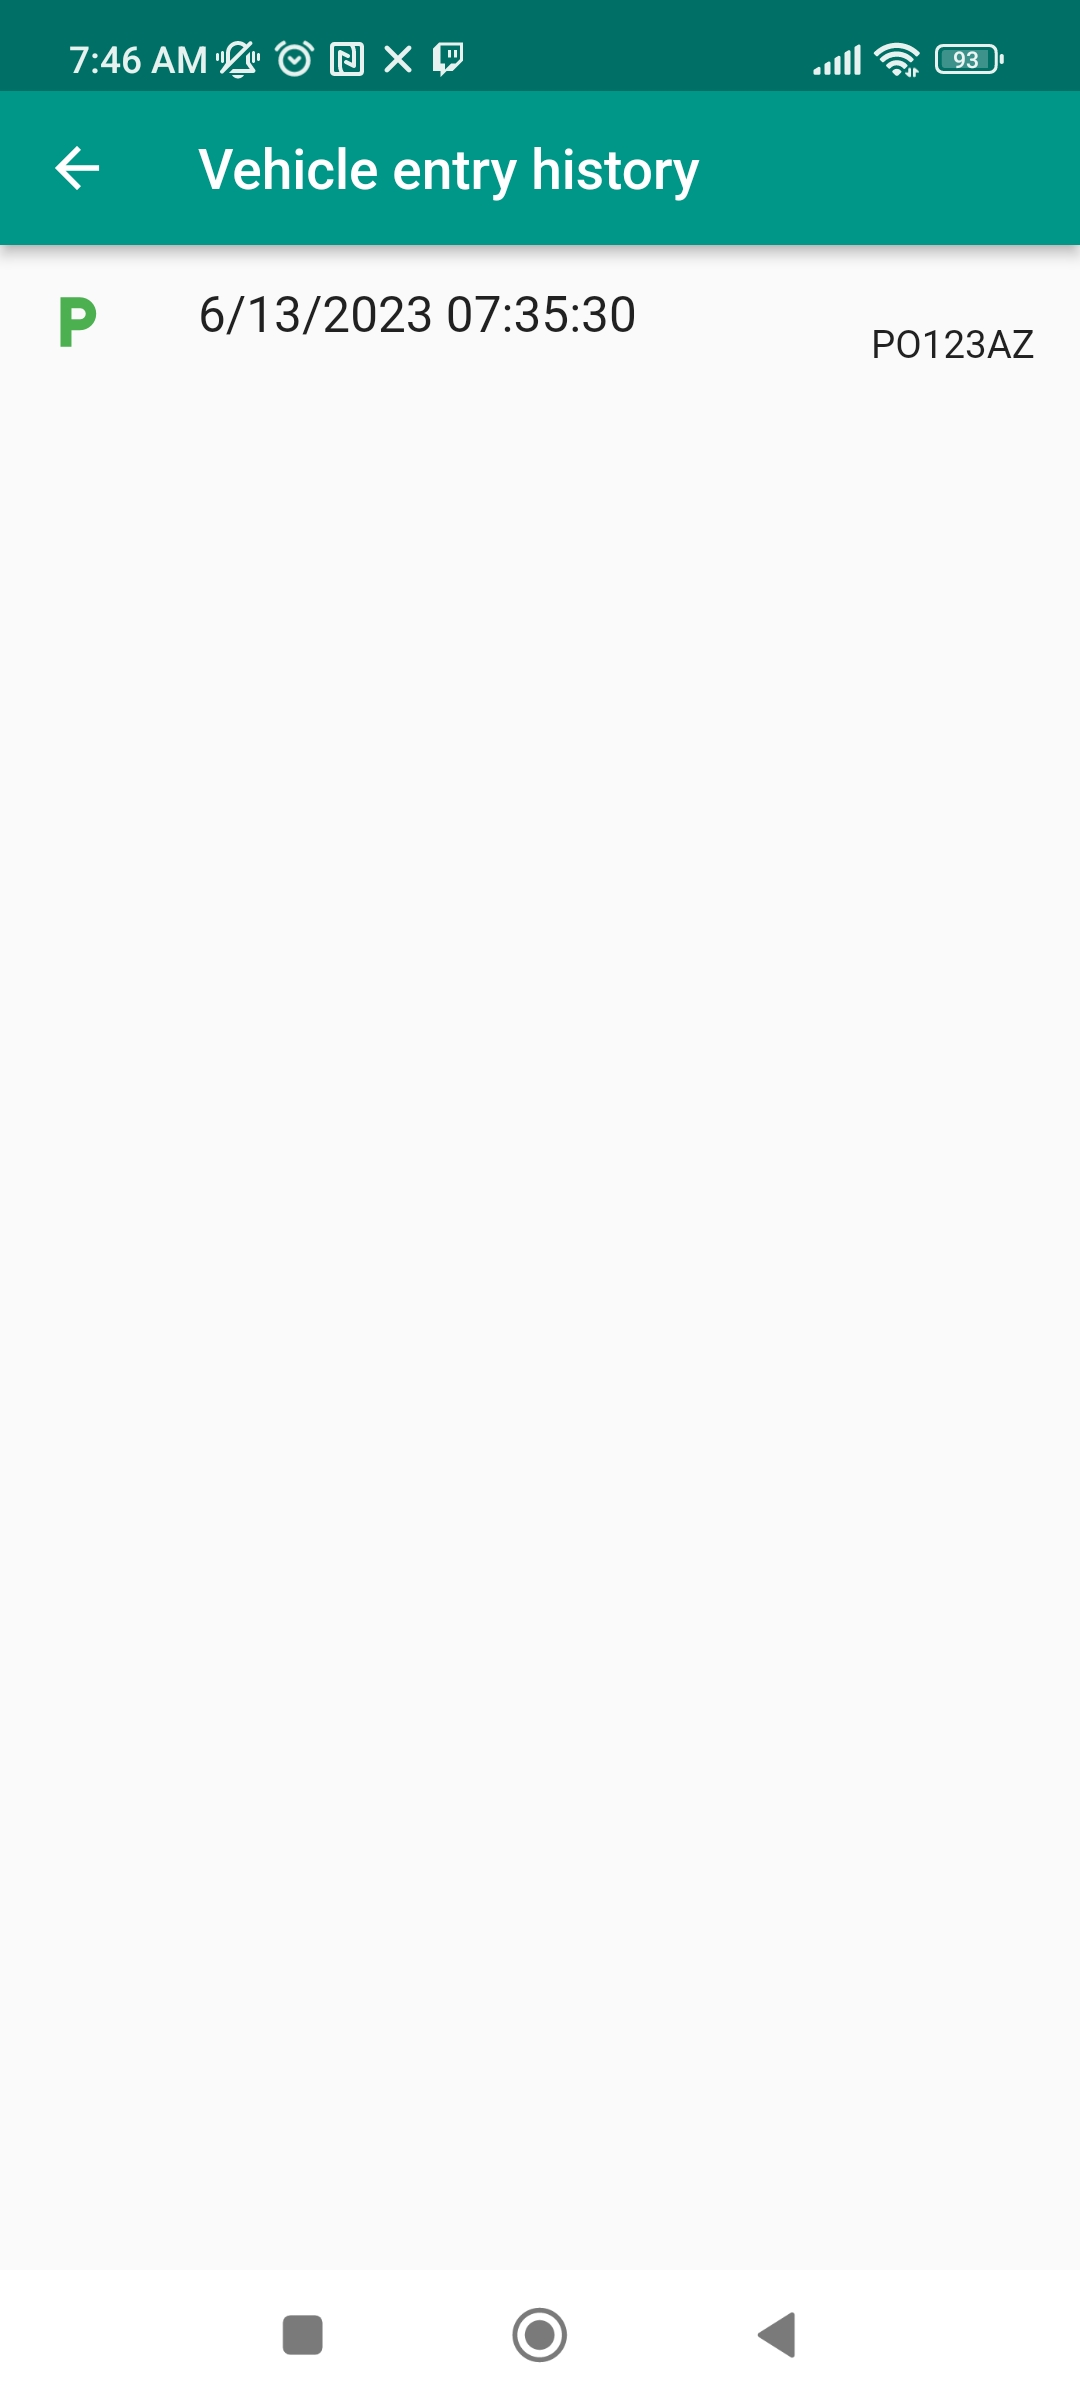
\includegraphics[width=0.6\linewidth]{oplacony.jpg}
\caption{Lista pojazdów znajdujących się na parkingu, za które została uiszczona opłata za postój.}
\end{center}
\end{figure}

\begin{figure}
\begin{center}
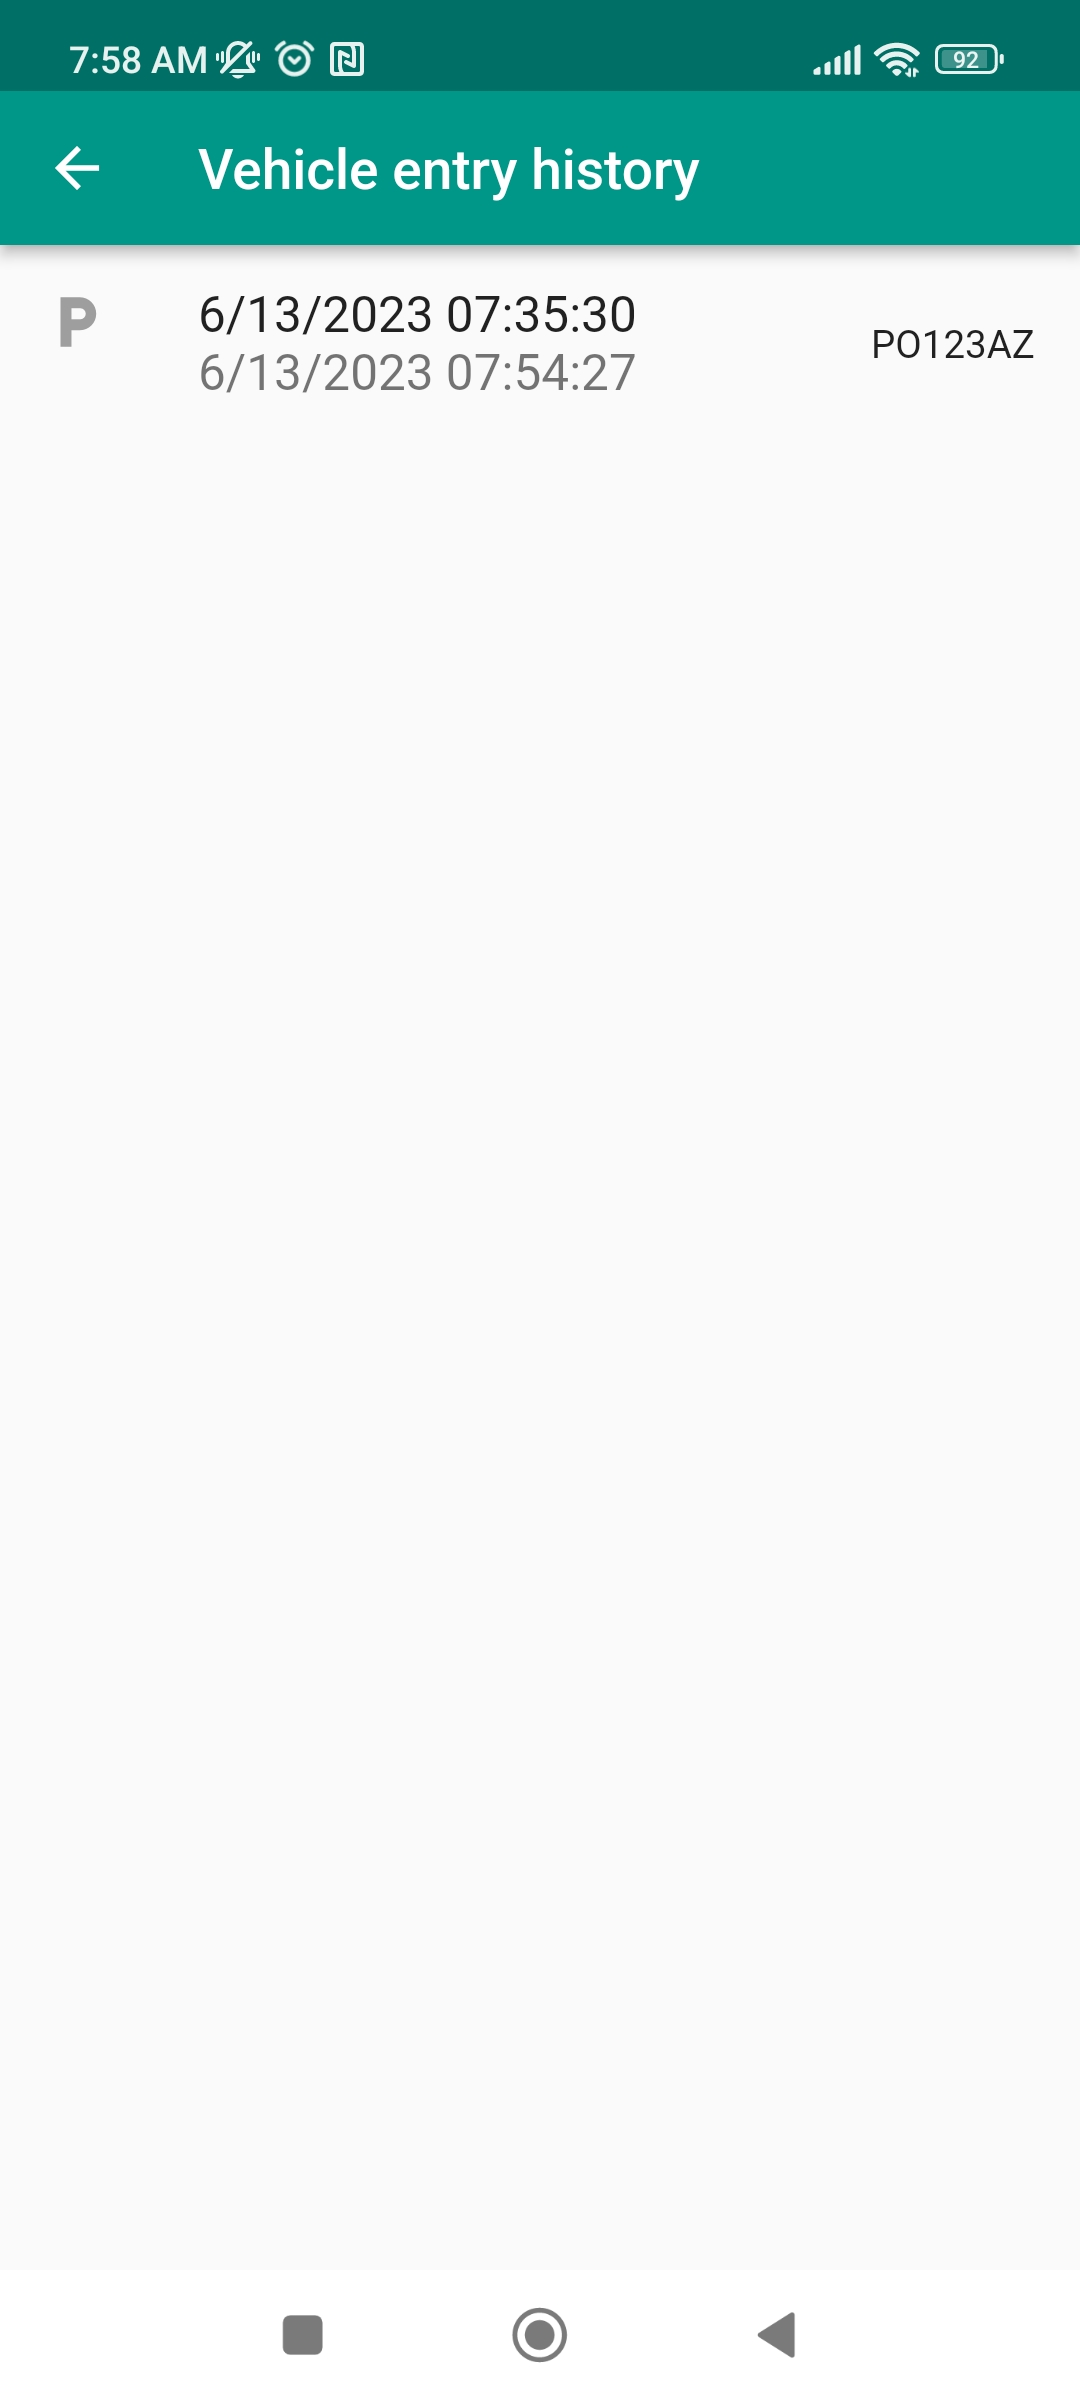
\includegraphics[width=0.6\linewidth]{zakonczony.jpg}
\caption{Lista pojazdów, które opuściły parking.}
\end{center}
\end{figure}




\end{document}